\documentclass[a4paper]{article}
\usepackage{ctex}
\usepackage[left=1.5cm, right=1.5cm, top=1.5cm, bottom=1.5cm]{geometry} %页边距
\usepackage{helvet}
\usepackage{amsmath, amsfonts, amssymb} % 数学公式、符号
\usepackage[english]{babel}
\usepackage{graphicx}   % 图片
%\usepackage{url}        % 超链接
\usepackage{bm}         % 加粗方程字体
\usepackage{multirow}
\usepackage{booktabs}
\usepackage{tikz}%调用宏包tikz
\usepackage{circuitikz}%调用宏包circuitikz
\usepackage{enumerate}
\usepackage{algorithm}
\usepackage{algorithmicx}
\usepackage{algpseudocode}
\usepackage{graphicx}
\usepackage[hidelinks]{hyperref}
\usepackage{listings}
\usepackage{textcomp}
\usepackage{multicol}
\usepackage[backend=biber,style=numeric,sorting=none]{biblatex}
\usepackage{setspace}
%\addbibresource{reference.bib}

% Python listing
\newcommand\pythonstyle{\lstset{
language=Python,
basicstyle=\sffamily,
keywordstyle=\textbf,
commentstyle=\color{blue},
showstringspaces=false, 
numbers=left }}
% Python environment
\lstnewenvironment{python}[1][]{
\pythonstyle \lstset{#1} }{}
\hypersetup{hidelinks,
	colorlinks=true,
	allcolors=blue,
	pdfstartview=Fit,
	breaklinks=true
    }
\newcommand{\threemetrics}[3]{\multirow{3}{*}{\shortstack[c]{$\textcolor{orange}{#1}$\\$\textcolor{blue}{#2}$\\$\textcolor{green}{#3}$}}}
\newcommand{\twometrics}[2]{\multirow{2}{*}{\shortstack[c]{$\textcolor{blue}{#1}$\\$\textcolor{green}{#2}$}}}

\renewcommand{\algorithmicrequire}{ \textbf{Input:}}       
\renewcommand{\algorithmicensure}{ \textbf{Output:}} 
%算法格式
\usepackage{subfigure}
\usepackage{fancyhdr} %设置页眉、页脚
\usepackage{gensymb}

\pagestyle{fancy}
\lhead{Digital signal processing}
\chead{}
\rhead{2024,Homework 3}
\lfoot{}
\cfoot{\thepage}
\rfoot{}
\linespread{2}

\usepackage{ifthen}
\usepackage{xifthen}

\newcommand{\dom}[1]{\mathop{\mathrm{dom}}\left(#1\right)}
\newcommand{\rng}[1]{\mathop{\mathrm{rng}}\left(#1\right)}
\newcommand{\preimg}[2][]{ \ifthenelse{\isempty{#1}}
    {\mathop{\mathrm{preimage}}\left(#2\right)}
    {\mathop{\mathrm{preimage}}_{#1}\left(#2\right)} }
\newcommand{\set}[1]{\left\{#1\right\}}

\newenvironment{proof}{{\par\noindent\it Proof.}\quad\par}{\hfill $\square$\par}  
\begin{document}
\section{Task 1}
We try to filt and retent 0-order light. We displayed ideal, butterworth and gaussian filter.
The cutoff frequency is set at 20, and displayed sine and rect mesh.\\
1. The sine mesh with frequency of $\dfrac{\pi}{4}$ and with ideal filter, with cutoff frequency 20.\\
\centerline{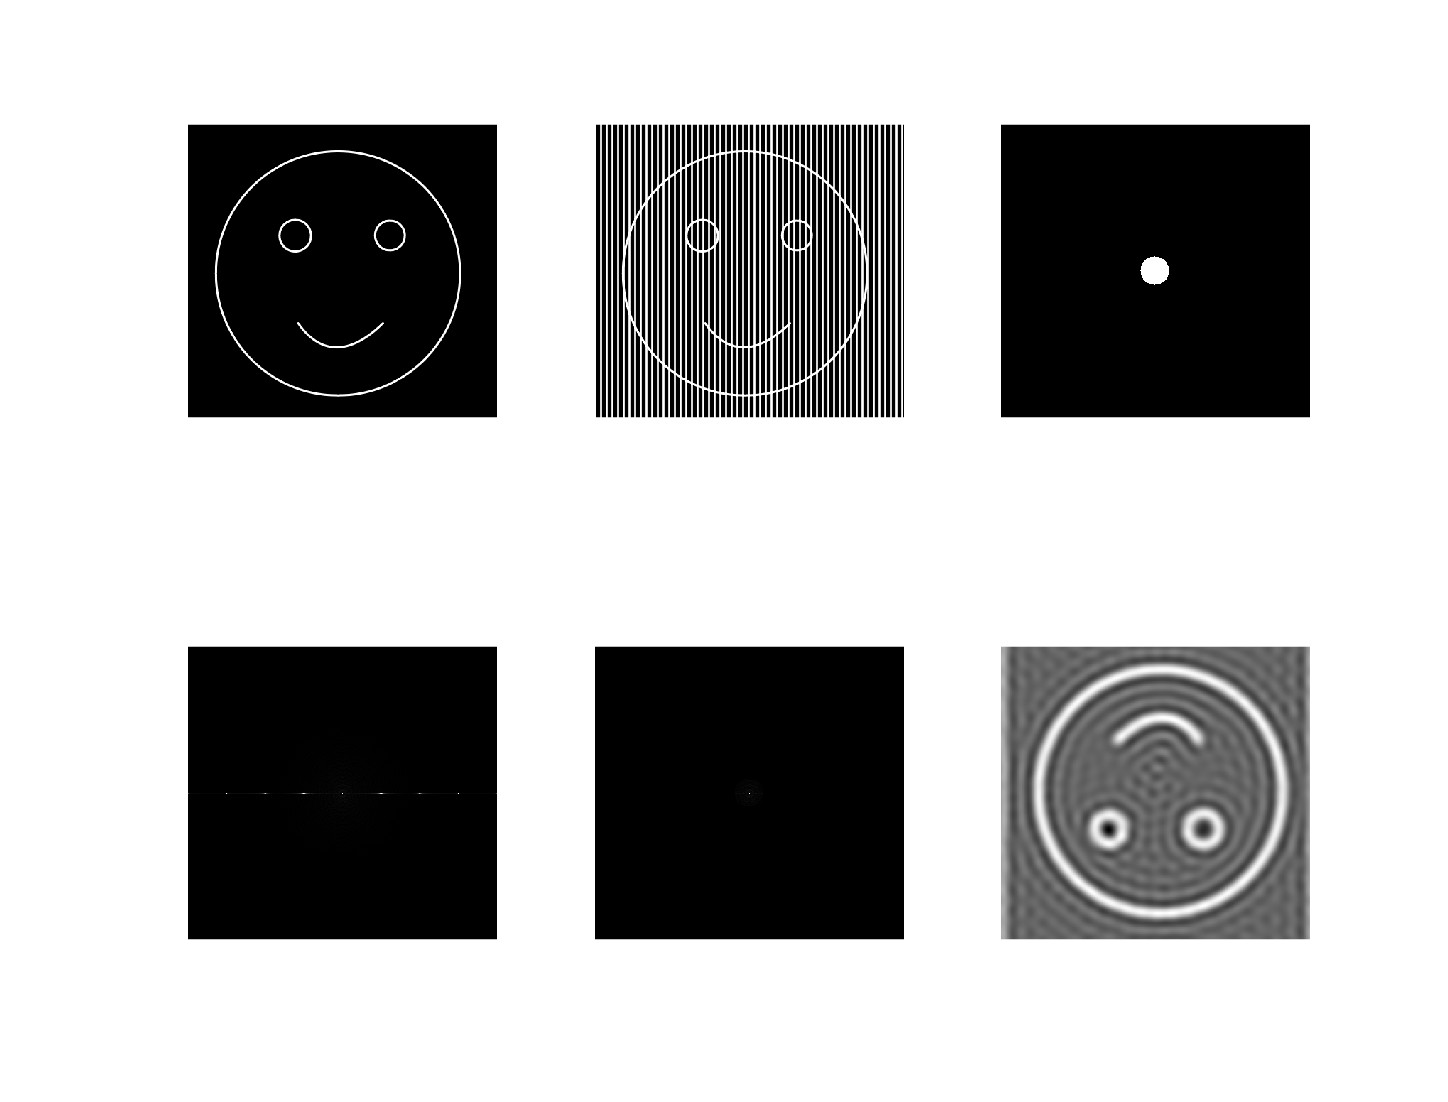
\includegraphics[scale=0.275]{1.jpg}}\\
2. The sine mesh with frequency of $\dfrac{\pi}{4}$ and with butterworth filter, with cutoff frequency 20, n=4.\\
\centerline{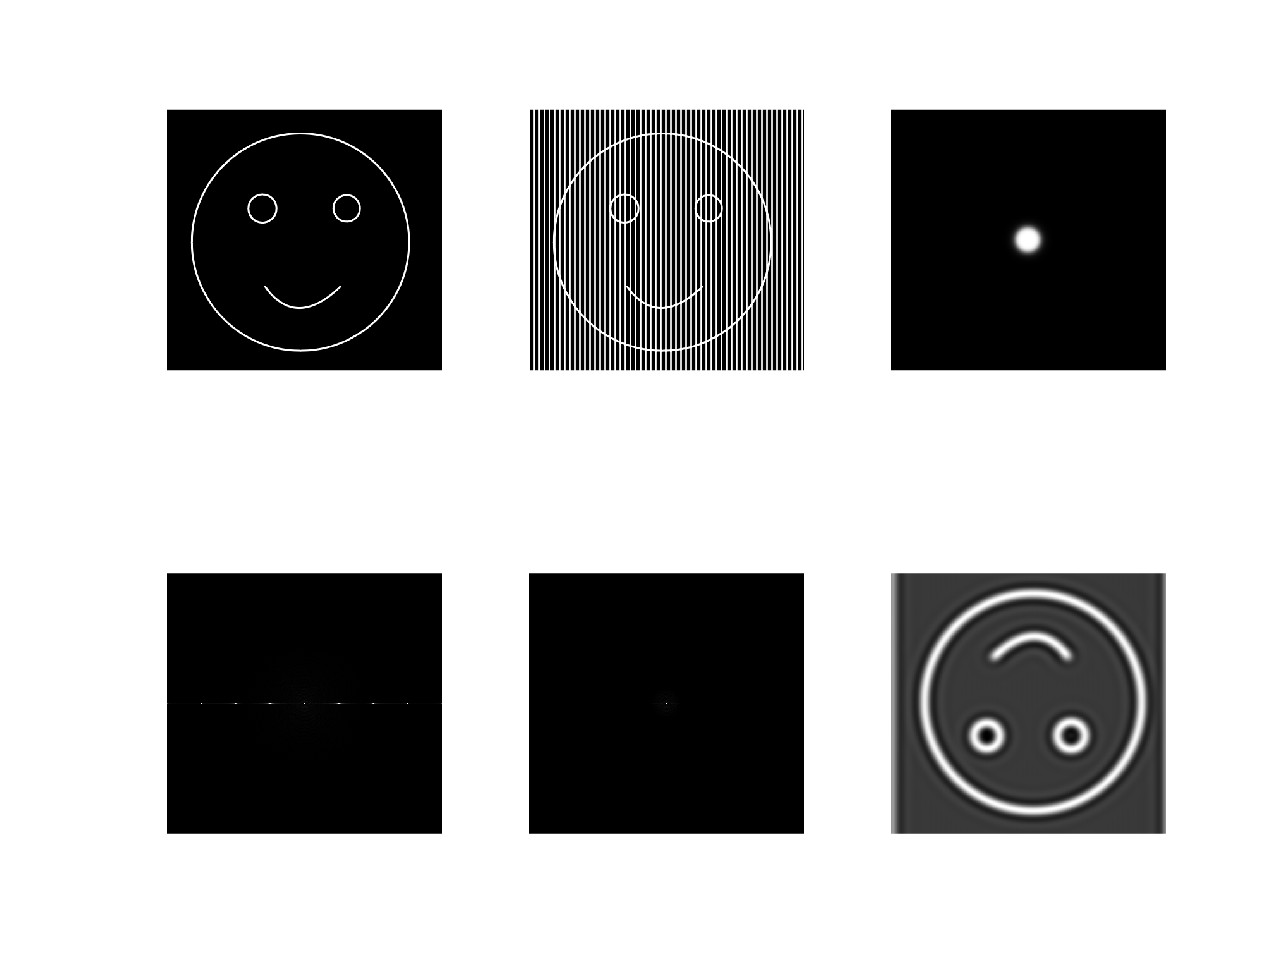
\includegraphics[scale=0.30]{2.jpg}}\\
The butterworth filter will approaches to ideal low pass filter by incrementing the factor n. Butterworth also 
smooth the incontinuous points at cut off frequency.\\
3. The sine mesh with frequency of $\dfrac{\pi}{4}$ and with gaussian filter, with cutoff frequency 10.\\
\centerline{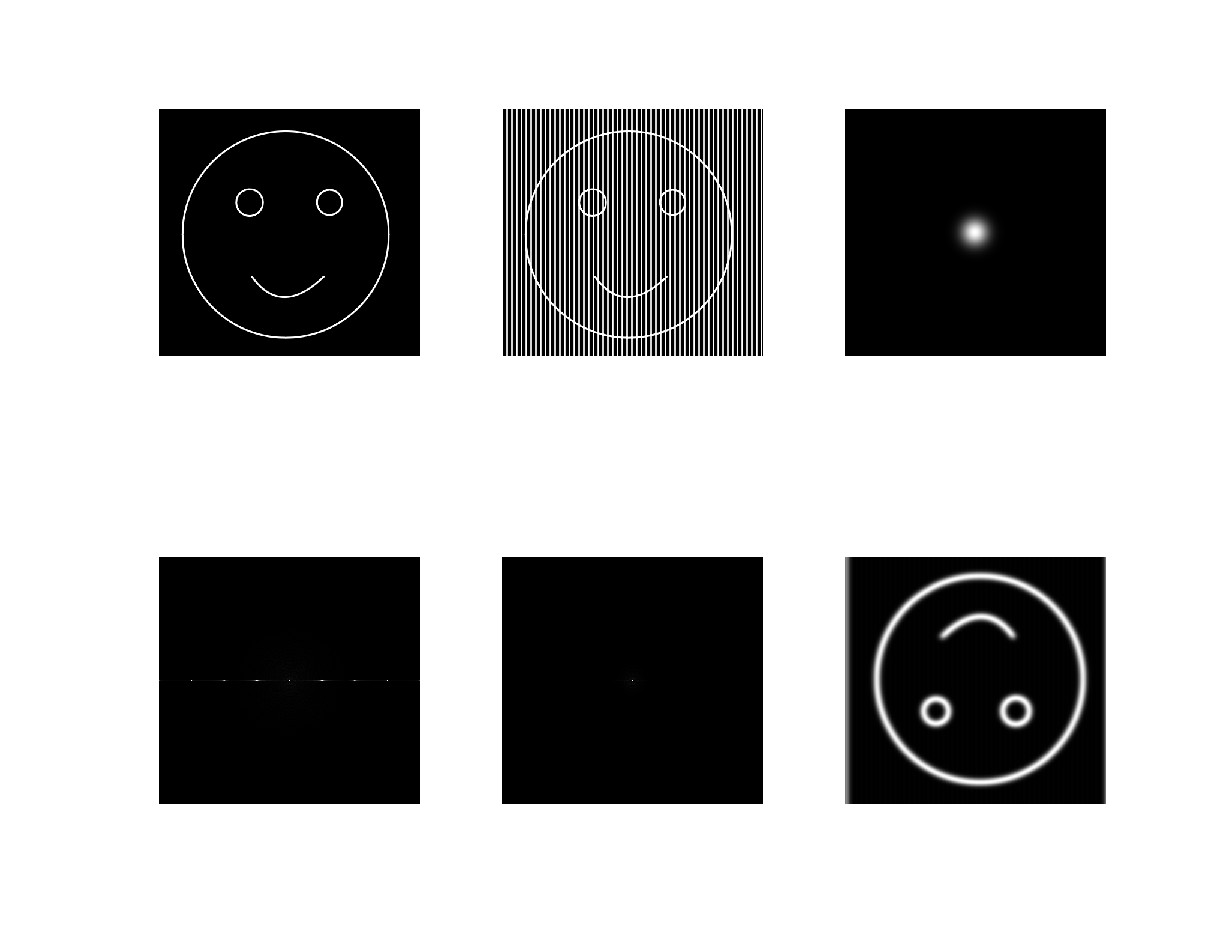
\includegraphics[scale=0.30]{3.jpg}}\\
Choose smaller frequency due to gaussian will keep little high frequency components. When too much Components are kept,
the streak is too obvious. Also, the smooth of gaussian makes it better than butterworth.\\
4. The rectangle mesh with period 10 and mod 4 with ideal filter. The cutoff frequency is 20.\\
\centerline{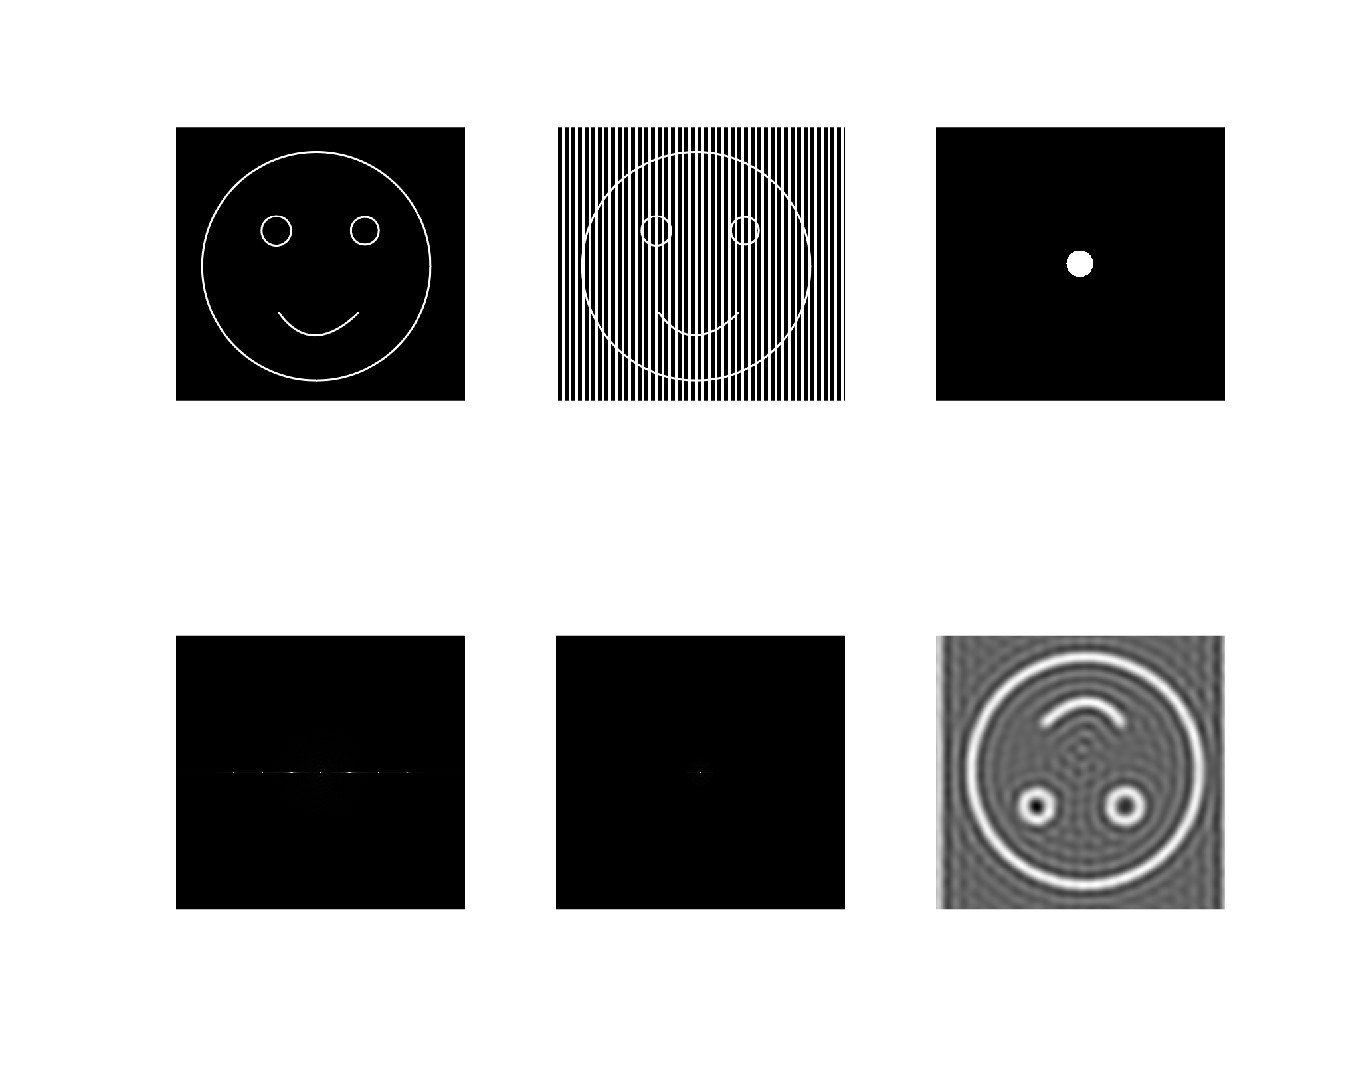
\includegraphics[scale=0.30]{4.jpg}}\\
5. The rectangle mesh with period 10 and mod 4 with butterworth filter. The cutoff frequency is 20, factor n=4.\\
\centerline{
\includegraphics[scale=0.30]{5.jpg}}\\
6. The rectangle mesh with period 10 and mod 4 with gaussian filter. The cutoff frequency is 10.\\
\centerline{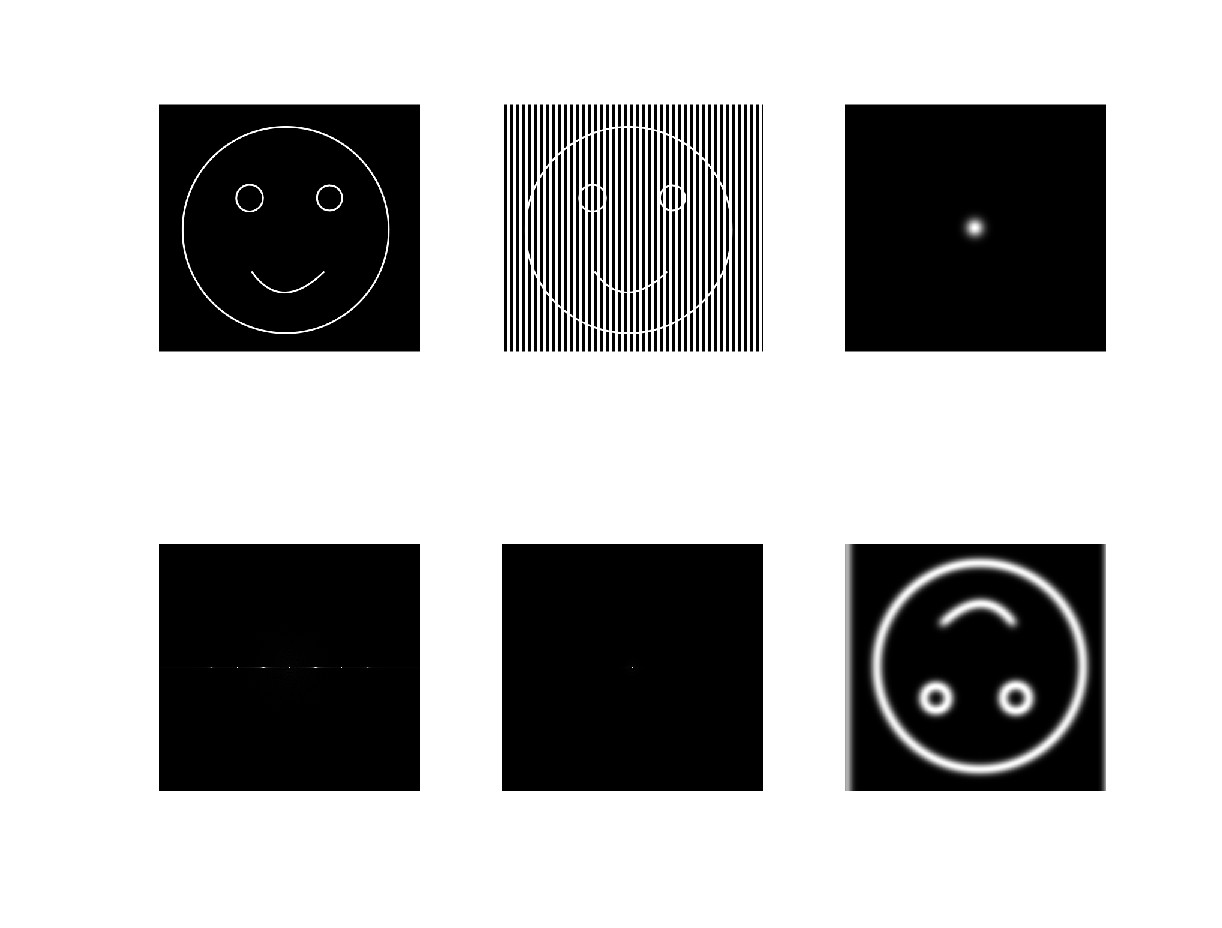
\includegraphics[scale=0.30]{6.jpg}}
\clearpage
\section{Task 2}
1. The sine mesh with frequency of $\dfrac{\pi}{4}$ and with ideal filter, with center at 60 and bandwidth of 40.\\
\centerline{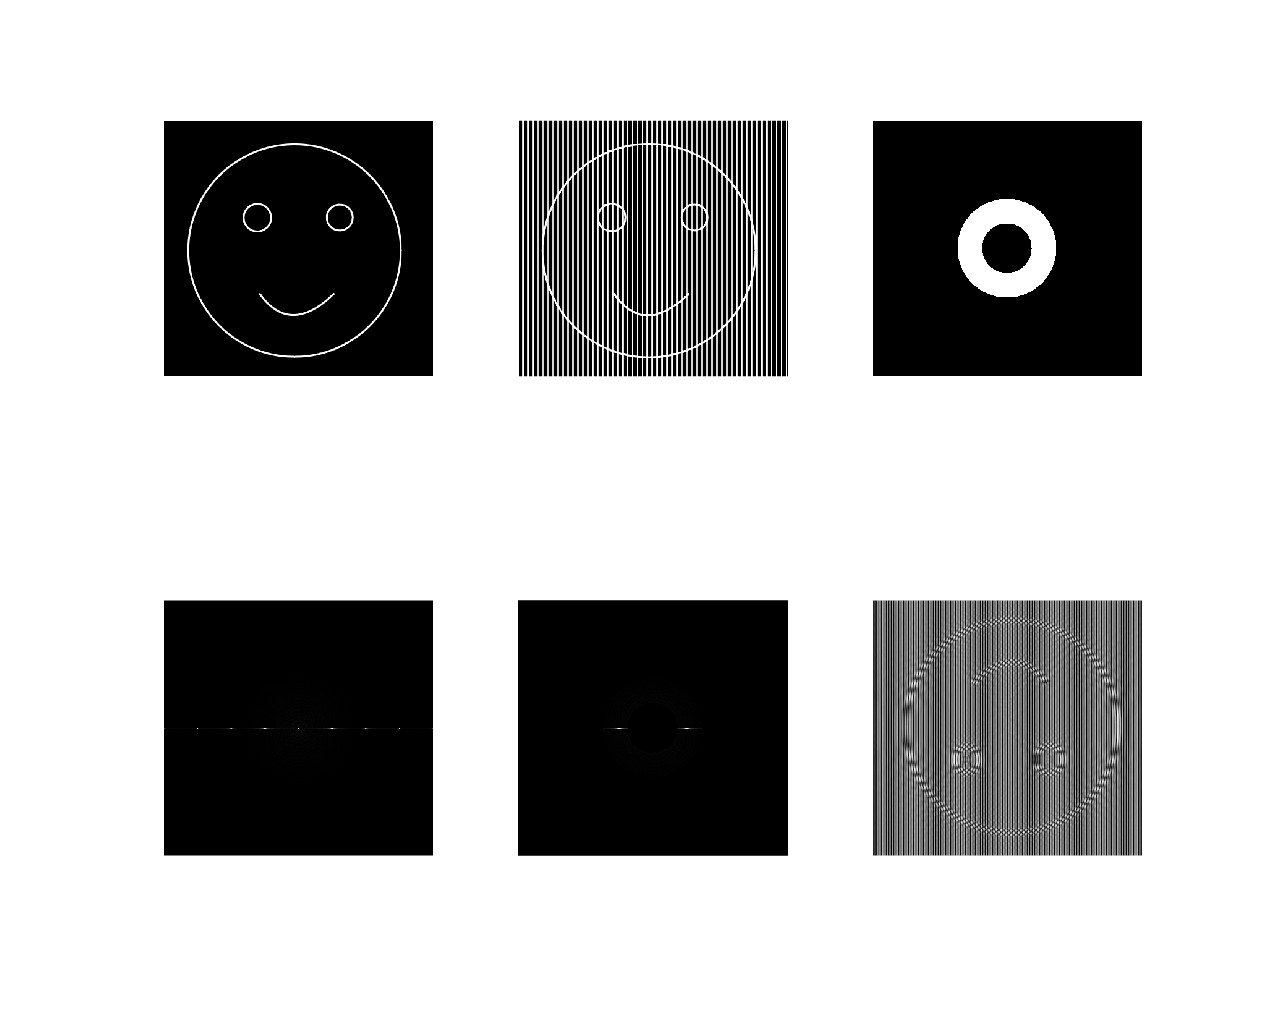
\includegraphics[scale=0.30]{7.jpg}}\\
2. The sine mesh with frequency of $\dfrac{\pi}{4}$ and with butterworth filter, with center at 60 and bandwidth of 40, factor n=4.\\
\centerline{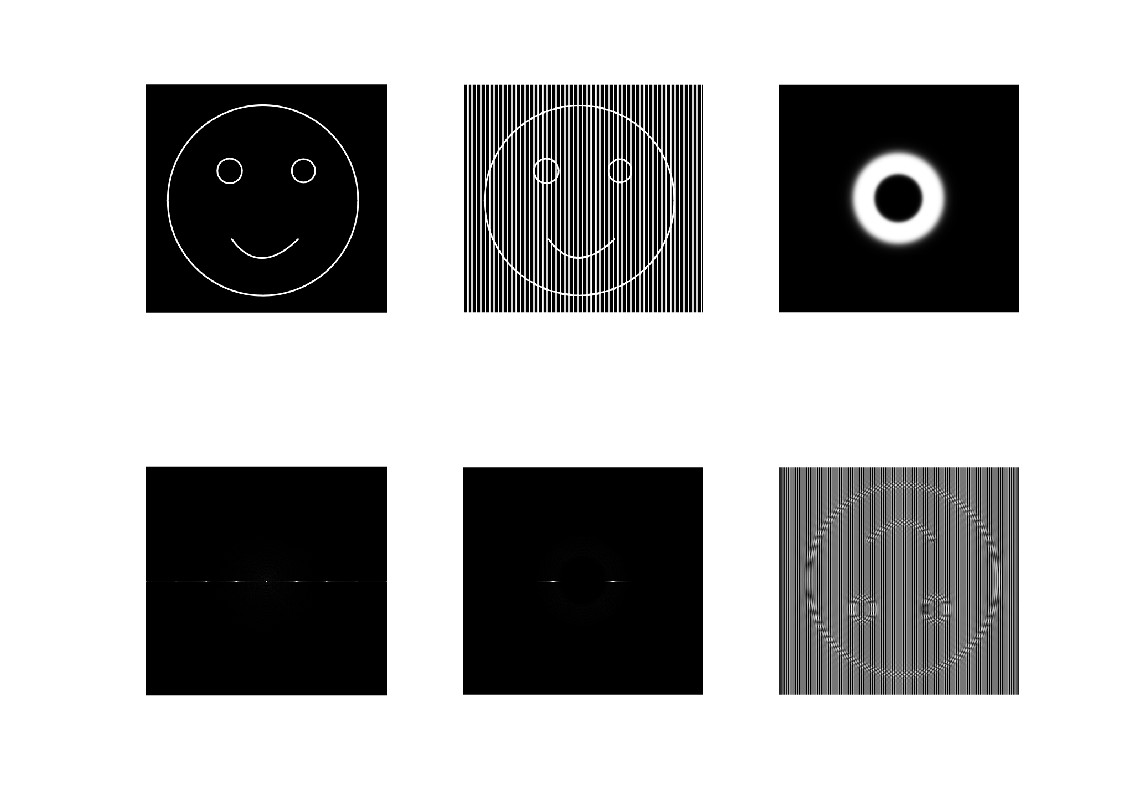
\includegraphics[scale=0.30]{8.jpg}}
\clearpage
3. The sine mesh with frequency of $\dfrac{\pi}{4}$ and with gaussian filter, with center at 60 and bandwidth of 40.\\
\centerline{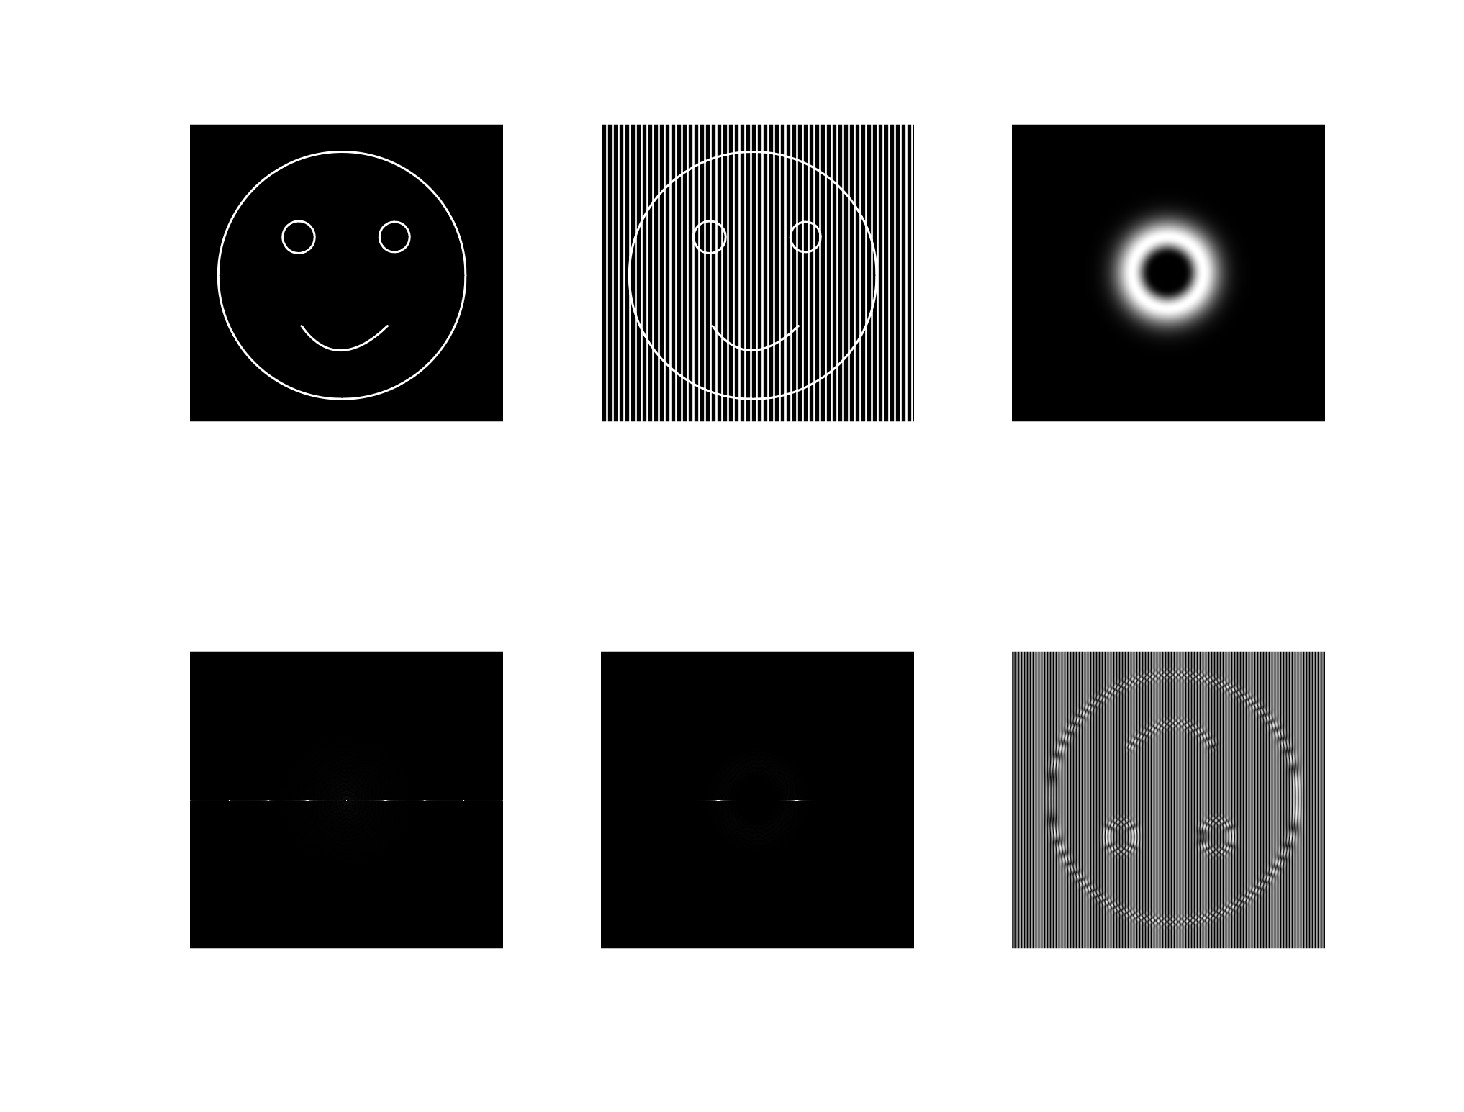
\includegraphics[scale=0.30]{9.jpg}}\\
4. The rect mesh with period 10 and mod 4 and with ideal filter, with center at 50 and bandwidth of 40.\\
\centerline{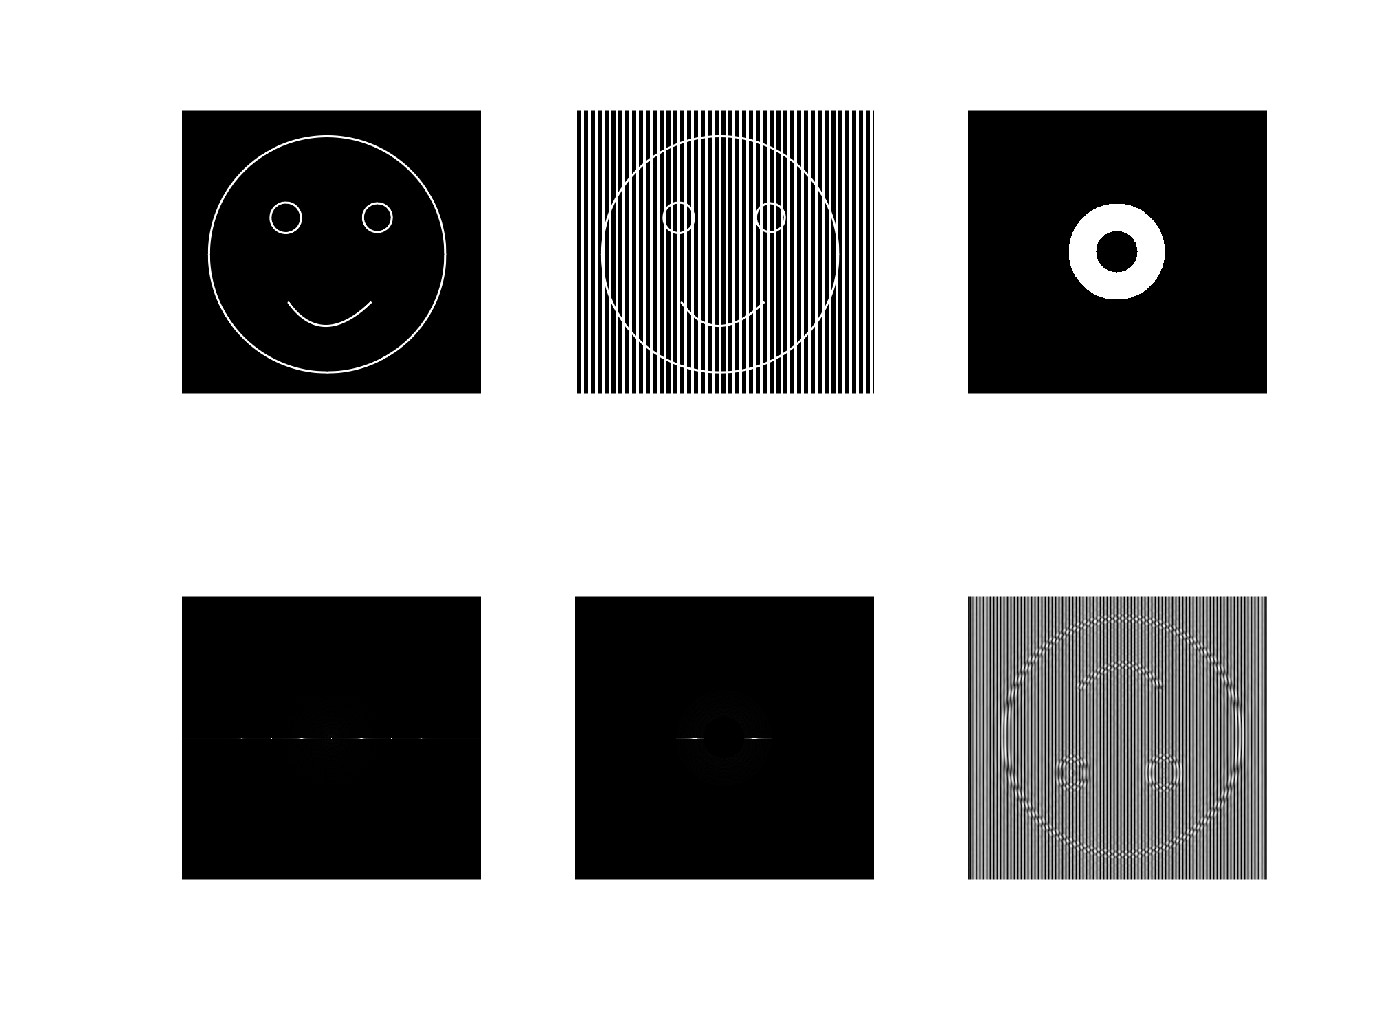
\includegraphics[scale=0.30]{10.jpg}}
\clearpage
5. The rect mesh with period 10 and mod 4 and with butterworth filter, with center at 50 and bandwidth of 40, factor n=4.\\
\centerline{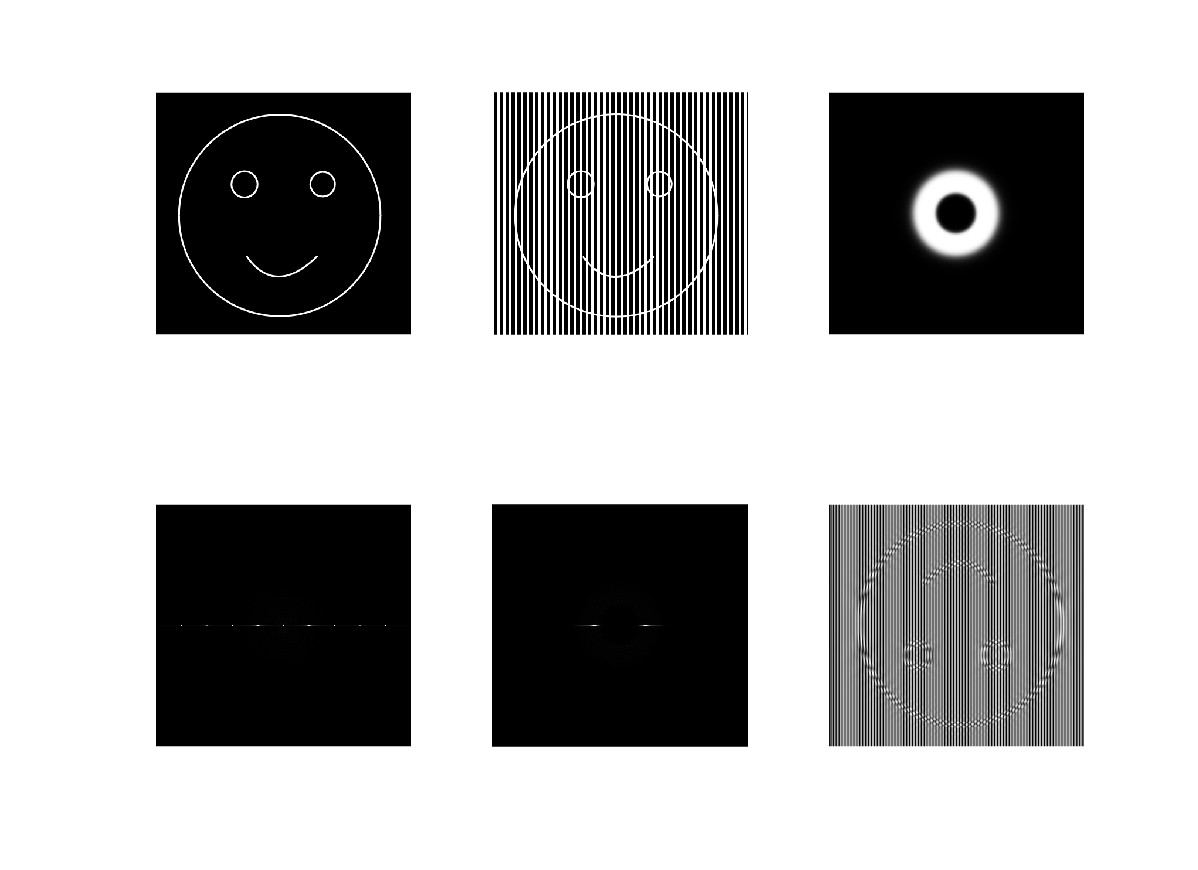
\includegraphics[scale=0.3]{11.jpg}}\\
6. The rect mesh with period 10 and mod 4 and with gaussian filter, with center at 50 and bandwidth of 40.\\
\centerline{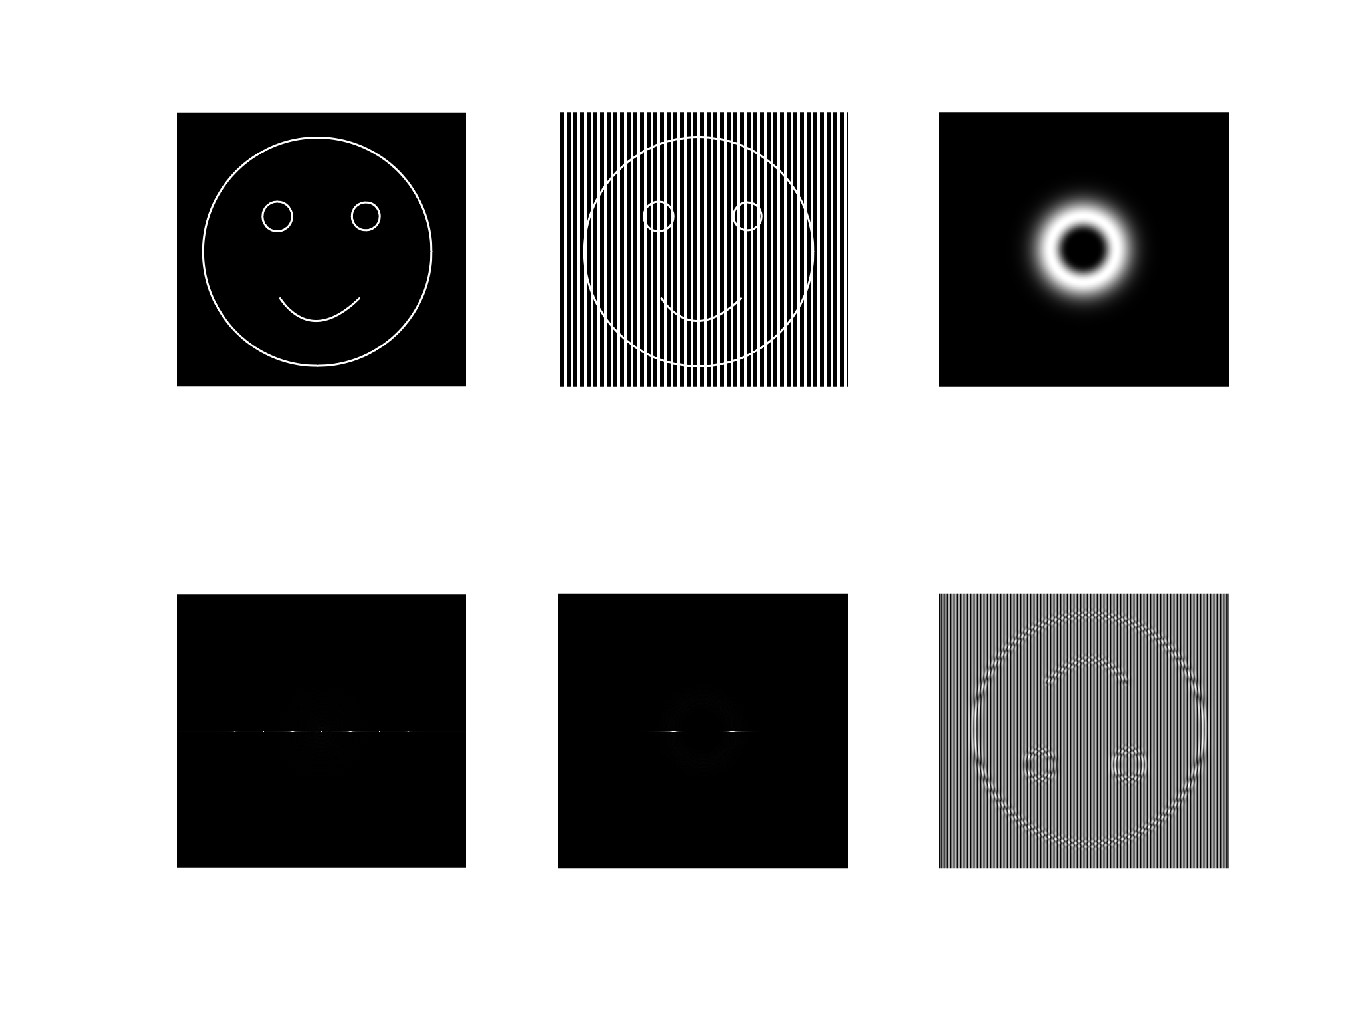
\includegraphics[scale=0.3]{12.jpg}}\\
I have packed the report with all matlab m functions for readers to re-experiment.
\end{document}